\documentclass[12pt]{report}

%%%% Load packages %%%%
\usepackage{geometry}                % See geometry.pdf to learn the layout options. There are lots.
\usepackage[parfill]{parskip}    % Activate to begin paragraphs with an empty line rather than an indent
\usepackage{graphicx}
\usepackage{tabularx}
\usepackage{graphics}
\usepackage{subfig}
\usepackage{epic}
\usepackage{ecltree}
\usepackage{amssymb}
\usepackage{hyperref}
\usepackage{epstopdf}
\usepackage[utf8]{inputenc}
\usepackage{amsmath}
\usepackage{fontenc}
\usepackage{boxedminipage}
\usepackage[T1]{fontenc}
\usepackage{xcolor}
\usepackage{babel} 

%%%% Load logo %%%%
\newcommand{\faclogo}{\protect
\includegraphics[height=25.9ex,keepaspectratio]{faclogo.png}}
\newcommand{\ilogo}{\protect
\includegraphics[height=25ex,keepaspectratio]{ilogo.jpg}}
\newcommand{\Rlogo}{\protect
\includegraphics[height=1.9ex,keepaspectratio]{Rlogo.png}}

%%%%%%%%Load des couleurs%%%%%%
\definecolor{bluemarine}{RGB}{0,102,204}
\definecolor{bluelight}{RGB}{204,255,255}
\definecolor{bluelight}{RGB}{186,213,240}
\definecolor{bluelight}{RGB}{228,233,239}
\definecolor{bleu_foncé}{RGB}{0,51,102}
\definecolor{bleu_moyen}{RGB}{0,102,153}

%%%% début réglage des packages%%%%%
\DeclareGraphicsRule{.tif}{png}{.png}{`convert #1 `dirname #1`/`basename #1 .tif`.png}
\setcounter{secnumdepth}{5} %augmenter la profondeur de numérotation
\geometry{a4paper}                   % ... or a4paper or a5paper or ... 
\textheight=25truecm
\textwidth=18truecm
\topmargin=-15truemm
\oddsidemargin=-10truemm
\evensidemargin=-10truemm 
%\geometry{landscape}                % Activate for rotated page geometry

%%%% macro-section %%%%
\makeatletter
\renewcommand{\thesection}{\arabic{section}. }
\renewcommand\section{\@startsection{section}{1}{\z@}%
	{1cm\@plus -1ex\@minus -0.2ex}%
	{1.3ex\@plus 0.2ex}%
	{\reset@font\Large\bf\sc}}
\makeatother

%%%% macro-subsection %%%%
\makeatletter
\renewcommand{\thesubsection}{\arabic{section}.\arabic{subsection} }
\renewcommand\subsection{\@startsection{subsection}{2}{\z@}%
	{1cm\@plus -1ex\@minus -0.2ex}%
	{1.3ex\@plus 0.2ex}%
	{\reset@font\large\bf}}
\makeatother

%%%% macro-subsubsection %%%%
\makeatletter
\renewcommand{\thesubsubsection}{\Alph{subsubsection}. }
\renewcommand\subsubsection{\@startsection{subsubsection}{3}{\z@}%
	{1cm\@plus -1ex\@minus -0.2ex}%
	{1.3ex\@plus 0.2ex}%
	{\reset@font\normalsize\bf}}
\makeatother

%%%% macro-paragraph %%%%
\makeatletter
\renewcommand{\theparagraph}{\alph{paragraph}) }
\renewcommand\paragraph{\@startsection{paragraph}{4}{\z@}%
	{1cm\@plus -1ex\@minus -0.2ex}%
	{1.3ex\@plus 0.2ex}%
	{\reset@font\normalsize\bf}}
\makeatother

%%%% macro-subparagraph %%%%
\makeatletter
\renewcommand{\thesubparagraph}{\roman{subparagraph}}
\renewcommand\subparagraph{\@startsection{subparagraph}{5}{\z@}%
	{1cm\@plus -1ex\@minus -0.2ex}%
	{1.3ex\@plus 0.2ex}%
	{\reset@font\normalsize\it}}
\makeatother

%%%% Other information %%%%
\title{Titre de la Revue}
\author{LIPINSKI Boris}
\date{Contrat d'alternance \\ Septembre 2020 à Aout 2021}                                           % Activate to display a given date or no date

\renewcommand{\contentsname}{Table des Matières}
\renewcommand{\listfigurename}{Table des Figures}

%%%%%%%%%%%%%%%%%%%%%%%%%%%%%%%%%%%%%%%%%%%%%%%%%%%%%%%%%%%%%%%%%%%%%%%%%%%%%%%%%%%%%%%%%%%%%%%%%%%%%%%%%%%%%%%%%%%%%%%%%%%%%%%%%%%%%%%%%%%%%%%%%%%%%%%%%%%%%%%%%%%%%%%%%%%%%%%%%%%%%%%%%%%%%%%%%%%%%%%%%%%%%%%%%%%%%%%%%%%%%%%%%%%%%%%%%%%%%%%%%%%%%%%%%%%%%%%%%%%%%%%%%%%%%%%%%%%%%%%%%%%%%%%%%%%%%%%%%%%%%%%%%%%%%%%%%%%%%%%%%%%%%%%%%%%%%%%%%%%%%%%%%
\begin{document}
\makeatletter

%%%%%page de présentation%%%%
\begin{titlepage}

%%%%%Logo fac%%%%
\begin{flushleft}
\faclogo
\end{flushleft}

%%%%%Logo inserm%%%%
\begin{flushright}
\vspace{-4.5cm}\ilogo
\end{flushright}

%%%%Cadre principale%%%%
\centering
\vfill
 
\fcolorbox{bleu_moyen}{white}{
\begin{minipage}{17cm}
\vspace{0.2cm}

\begin{center}
\LARGE \textbf{{Rapport de Stage : Projet Flinovo \\ Analyses en single cell des réponses de patients atteint de lymphome folliculaire à un traitement, le RCHOP.}} 

\end{center}

\vspace{0.2cm}
\end{minipage}}

%%%%Cadre secondaire%%%%
\vspace{4cm}
\LARGE\@author \\
\vspace{1cm}   
\Large\@date\   
\vfill

\begin{flushleft}

\normalsize{
\textbf{Maitre d'apprentissage :} SUJOBERT Pierre \\
\textbf{Tuteur pédagogique :}  BROCHIER Céline \\
\textbf{Entreprise d'acceuil :} Laboratoire UR LIB « Lymphoma Immuno-Biology », Équipe Gilles Salle.\\
\textbf{Etablissement :} Université de Claude Bernard Lyon 1, Faculté de Médecine Lyon-Sud.\\
\textbf{Formation :} Master 2 Bioinformatique Moléculaire, Méthodes et Analyses. 
}

\end{flushleft}
\end{titlepage}

\let\original@addcontentsline\addcontentsline
\newcommand{\dummy@addcontentsline}[3]{}
\newcommand{\DeactivateToc}{\let\addcontentsline\dummy@addcontentsline}
\newcommand{\ActivateToc}{\let\addcontentsline\original@addcontentsline}
\makeatother

%%%%%%%%%%%%%%%%%%%%%%%%%%%%%%%%%%%%%%%%%%%%%%%%%%%%%%%%%%%%%%%%%%%%%%%%%%%%%%%%%%%%%%%%%%%%%%%%%%%%%%%%%%%%%%%%%%%%%%%%%%%%%%%%%%%%%%%%%%%%%%%%%%%%%%%%%%%%%%%%%%%%%%%%%%%%%%%%%%%%%%%%%%%%%%%%%%%%%%%%%%%%%%%%%%%%%%%%%%%%%%%%%%%%%%%%%%%%%%%%%%%%%%%%%%%%%%%%%%%%%%%%%%%%%%%%%%%%%%%%%%%%%%%%%%%%%%%%%%%%%%%%%%%%%%%%%%%%%%%%%%%%%%%%%%%%%%%%%%%%%%%%%
\begin{minipage}{\textwidth}
\section*{Résumé}
\tableofcontents
\listoffigures
%\vspace{6cm}
\section{Liste des abréviations utilisées}
\begin{itemize}
\item item 1
\end{itemize}
\end{minipage}

\section{Liste des logiciels utilisés}
\begin{itemize}
\item \Rlogo : 4.0.5 (2021-03-31) Shake and Throw
\begin{itemize}
\item Seurat : 4.0.0
\item SingleR : 1.4.1
\item celldex : 1.0.0
\item scRNAseq : 2.4.0
\item CellSIUS : 1.0.0
\item ggplot2 : 3.3.3
\item plotly : 4.9.3
\item shiny : 1.6.0
\item shinyjs : 2.0.0
\item shinydashboard : 0.7.1
\item Signac : 1.1.1
\item scone : 1.14.0
\item escape : 1.1.1
\item dittoSeq : 1.2.5
\item shinyWidgets : 0.5.7
\item monocle : 2.18.0
\item cowplot : 1.1.1
\item scran : 1.18.5
\item clues : 0.6.2.2
\item TENxBUSData : 1.4.0
\item dplyr : 1.0.5
\item tidyverse : 1.3.0
\end{itemize}
\item Python : 3.8.3
\begin{itemize}
\item pandas : 1.1.4
\item plotly : 4.14.3
\item seaborn : 0.11.1
\item numpy : 1.19.4
\item scipy : 1.5.4
\item matplotlib : 3.3.2
\item jupyter-notebook : 6.2.0
\end{itemize}
\item CellRanger : count, VDJ
\item CITE-SEQ count :
\item IronThrone-GoT : 2.1
\end{itemize}


%%%%%%%%%%%%%%%%%%%%%%%%%%%%%%%%%%%%%%%%%%%%%%%%%%%%%%%%%%%%%%%%%%%%%%%%%%%%%%%%%%%%%%%%%%%%%%%%%%%%%%%%%%%%%%%%%%%%%%%%%%%%%%%%%%%%%%%%%%%%%%%%%%%%%%%%%%%%%%%%%%%%%%%%%%%%%%%%%%%%%%%%%%%%%%%%%%%%%%%%%%%%%%%%%%%%%%%%%%%%%%%%%%%%%%%%%%%%%%%%%%%%%%%%%%%%%%%%%%%%%%%%%%%%%%%%%%%%%%%%%%%%%%%%%%%%%%%%%%%%%%%%%%%%%%%%%%%%%%%%%%%%%%%%%%%%%%%%%%%%%%%%%
\section{Section principale}
\subsection{Introduction}

Une introduction présentant l'état de l'art et le contexte scientifique dans lequel s'inscrit le travail réalisé ainsi que la(les) problématique(s) abordées pendant le stage ;

De nombreux processus sont impliqués dans le développement et l’évolution du cancer. L’expansion de cellules tumorales dans l’organisme va de pair avec l’accumulation d’altérations génétiques induites par mutations somatiques.


\subsubsection*{Contexte scientifique}

Le cancer se caractérise par l'apparition de cellules qui échappent aux systèmes de contrôle de cycle cellulaire.
Ces cellules dites tumorale acquiescent la capacité à proliférer de façon incontrolée, leur progression et leur adaptation à l'environnement suivent principalement des processus évolutifs. 
Il est généralement accepté que les cellules tumorales sont issues d’une seule cellule donnant lieu à des sous-populations caractérisées par l'accumulation de nombreuses nouvelles altérations génétiques. 
En effet, génération après génération la diversité génétique au sein de la population cellulaire tend à s'accroitre par acquisition successive de mutations somatiques
[McGranahan N. et Swanton C. Biological and therapeutic impact of intratumor heterogeneity in cancer evolution. Cancer Cell, 27(1) :15 – 26, 2015.] pouvant favoriser l'apparition de cellules de plus en plus disfonctionnelles. 
Ainsi certaines cellules s'écartent des processus physiologiques standards jusqu'à échaper à l'immuno-surveillance, les rendants donc potentiellement précurseures de tumeurs cancéreuses malignes. 
De ce fait, le cancer découle de dynamiques cellulaires et moléculaires complexes et anormales, suivant des modèles d’expansion clonale et de diversité très variable à la fois selon le type de cancer et selon l’individu. 

Parmis les différents types de cancers se trouve le diagnostique du lymphome folliculaire, une tumeur maligne incurable des lymphocyte B qui compte pour 25\% des lymphomes, soit le 2ème lymphome par ordre de fréquence. 
La manifestation des symptomes cliniques est en grande partie indolore, s'exprimant principalement via gonflements des ganglions lymphatiques dans les régions du cou, des aisselles ou de l’aine. 
En dépit des progrès récents de notre compréhension sur la physiopathologie de ce cancer [papier Sarah huet], cette maladie est toujours concidérée comme étant incurable, et la plupart des patients atteints en décède des années après le diagnostique. 

Administrer un traitement revient toujours à être délicat quelque soit le cancer diagnostiqué. 
Au delà des effets curatifs thérapeutiques primaire et secondaires connus et attendus, le résultat peut tout aussi se révéler être inatendu, amplifiant une certaine progression tumorale pour des lignées cellulaires résistantes,
favorisée par pressions de sélections et donc éliminant progressivement toutes autres cellules sensibles au traitement [2]. 
Ainsi une adaptation et une résistance au traitement des sous-populations cellulaires déjà existantes peut apparaitre par sélection darwinienne, phénomène souvent grandement impliqué dans l’échec thérapeutique. 

Dans le contexte du lymphome folliculaire, il a été montré que la majorité des patients parviennent à une rémission complète s'ils sont soumis au traitement composé à base de RCHOP, 
ensemble de 5 molécules thérapeutiques : Rituximab, Cyclophosphamide, Hydroxyadrimycine, Vincristine et Prendisone [papier gille salle]. 
Cependant, un gand nombre de patient ont été victimes de rechute post-traitrement pouvant mener jusqu'a la mort, principalement à cause de toxicités liées au traitement même ou bien à une progression incontrolable et inatendue de la malaide (Hiddemann and cheson).

Caractériser et prédire au mieux la réponse clinique au traitement consititue donc un des enjeux majeur lié à cette problématique biologique. 
Cela pourrait se montrer être décisif dans la compréhension de l'évolution tumorale face au traitement, afin de maximiser à terme les chances de guérison des patients.

De nos jours, il est d’ores et déjà possible d'entrevoir que des analyses nécessitant un tel degré de précision soit réalisable. 
En effet, l’efficacité technologiques des méthodes d’analyse en single-cell est telle qu’elles permettent de caractériser les populations cellulaires intra-tumorale au plus haut degré de précision possible, tant au niveau ADN qu’ARN. 

Les outils de RT-qPCR ont d'abord montré que le single-cell peut être utilisé pour étudier les changements d’expressions par gènes et par cellules au cours de la différentiation embryonnaire [9].  
L'évolution complexe de populations cellulaires à aussi pu être caractériser par méthode de séquençage et d’analyse cellulaire RNA-seq en single-cell, permettant l'observation de trajectoires de différenciation de lignées distinctes, 
de l’hétérogénéité transcriptionnelle associée au cycle cellulaire et des programmes cellulaires de résistance aux médicaments impliqués [10] [11].
La profondeur analytiques que permettent les technologies en single cell semblent donc tout à fait pertinante pour apporter des éléments anlytiques à la fois vastes, précis et cohérant avec notre problématique.

L'utilisation du single cell impose l'optimisation du séquençage lui-même par l'utilisation d'identificateurs moléculaires uniques (UMI). 
L’incorporation d’un barcode dans l’étape de reversetranscription du séquençage permet d'assigné chaque read séquencé issus de transcrits exprimés à la cellule d’origine.  
La précision du comptage de transcrits et la reproductibilité de quantification en single-cell s'en retrouve donc bien meilleur, tout en supprimant efficacement les biais de réplicats induit par la PCR, vecteur de surexpression génique factice [10].
C’est ainsi que des comportements et sous-types de populations cellulaires peuvent être identifiés sur la base d’observation des résultats d’analyses transcriptomiques. [11][12]

C'est en prenant partie de avancées téchnologiques que des industries tels que 10X Genomics ont put de s'agrandir, mettant toujours à diposition des technologies de séquençage de pointes utilisable pour la recherche scientifique, notemment en signel cell. 
Les outils analytiques proposés par 10X Genomics permettent l'investigation d'analyse intégrative en single cell de population tumorales à des niveaux phénotypiques, transcriptomiques et génétiques, 
et leur application se trouve donc être en adéquation parfaite notre projet.

C’est dans ce contexte biologique que se projette le travail effectué pendant ce contrat d'alternance, illustrant le lancement d'un projet appelé FLINOVO. 
Comprendre et quantifier l'ampleur des effets du RCHOP sur des patients constitue notre problématique et nécessite de comparer l'état des mêmes cellules avant et après traitement.
Ainsi cette étude souhaite inclure à terme l'analyse 30 patients atteints du cancer du lymphome folliculaire soumis au RCHOP, parmis lesquels 2 réponses cliniques ont principalement été observées : 
14 patients ont eu une réponse favorable au traitement sans rechute par la suite, 16 ont eu une réponse partielle et/ou une rechute rapide de la maladie.
L'application d'un nouveau modèle expérimental basé sur la xénogreffe in ovo de cellules d'intérêts sur des embryons de poulets permettant simultanément d'obserser l'état des cellules soumises et non soumise au traitement.
L'hypothèse tester ici est de savoir si la xénogreffe in ovo permet de prédir la réponse clinique au traitement, et constitue le coeur de la problématique de ce projet et de ce rapport. 

\subsubsection*{Problématiques abordées pendant le stage}
Prédir la réponse clinique au traitement de patients atteint de lymphome folliculaire et en soutirer des corrélations nécessite l'élaboration d'un protocole analytique bioinformatique à la fois vaste et profond,
incluant le plus faible biais de variabilité technique possible et maximisant l'expression de la variabilité biologique d'intérêt. 

D'une manière globale, cela demande de savoir manipuler dfférents language de programation, adapter des scripts executables sur des clusters à hautes perfomrances,
mais aussi d'avoir le recul nécessaire pour choisir pertinemment les outils et techniques d'analyses, de normalisation et de réduction de dimensions adéquates à nos données, notre méthode et notre problématique.
D'autre part et plus précisément, de nombreuses recherches complémentaire sont nécessaire de manière à donner la plus grande profondeur possible à nos analyses. 
Ce travail d'approfondissement divise notre objectif en plusieurs taches concrètes nécésitant à la fois d'être en mesure de reproduire des analyses issues de la littérature mais aussi de pouvoir se les approprier. 

Le but est donc tout d'abord de mettre en évidence les résultats d'observations et comparaisons des tendances d'expression géniques issues des analyses en single-cell des différentes populations phénotypiques cellulaires pour chaque patient intra et inter groupes cliniques.
Ces résultats se complètent grace à des analyses d'enrichissements de gènes afin d'éclaircir la nature des fonctions cellulaires les plus impactées entre les 2 groupes de patients.
En parallèle, il s'agit aussi de mettre en place le génotypage du transcriptome à l'échelle de la cellule unique de hotspot d'intérêt présent dans certains gènes à tendance anti-apoptotique ou oncogène qui joueraient un rôle déterminant dans l'apparition de lymphome folliculaire.
La détectection et la quantification de la présence des différentes populations de récepteurs BCR au sein des populations polyclonales des lymphocytes B issus des populations cellulaires tumorales est aussi à réaliser en tandem, 
tout comme l'analyse de l'état du cycle cellulaire dans lequel ces dernières se trouvent.

La superposition de l'ensemble de ces informations et d'autres pour chacunes des cellules d'intérêt constitues aussi en soi une tache à réaliser, relatant d'un aspect plus technique que biologique. 
Cette dernière tache introduit la nécéssité d'abordé la problématique de clusterisation et de réduction de dimenstion de notre jeu de données, afin d'identifier quelles informations expliquent le plus de variance. 
De plus, il est nécessite de mettre en place des outils analytiques purement technique de manière à rendre la réalisation la visualisation des analyses simples, facilement compréhensible, automatisable et à la porté de biologiste et médecin non bio-informaticien.
Dans le prolongement des taches techniques, des compétences purement informatiques sont requise. L'identification pertinante des ressources CPU, RAM et stockage à dû être nécessaires afin de rendre les analyses réalisable, 
car un tel projet basé sur l'utilisation des technologies en single cell amène forcément à la génération d'un grand nombre de données extrêmement volumineuse.

Enfin de part la nature purement exploratoire du projet et le fait qu'aucun résultat à priori n'est attendu, les taches décrites ci-dessus sont et seront amenées à évoluer.
De plus d'autres restent encore déterminables en fonction de l'évolution du projet.




%%%%%%%%%%%%%%%%%%%%%%%%%%%%%%%%%%%%%%%%%%%%%%%%%%%%%%%%%%%%%%%%%%%%%%%%%%%%%%%%%%%%%%%%%%%%%%%%%%%%%%%%%%%%%%%%%%%%%%%%%%%%%%%%%%%%%%%%%%%%%%%%%%%%%%%%%%%%%%%%%%%%%%%%%%%%%%%%%%%%%%%%%%%%%%%%%%%%%%%%%%%%%%%%%%%%%%%%%%%%%%%%%%%%%%%%%%%%%%%%%%%%%%%%%%%%%%%%%%%%%%%%%%%%%%%%%%%%%%%%%%%%%%%%%%%%%%%%%%%%%%%%%%%%%%%%%%%%%%%%%%%%%%%%%%%%%%%%%%%%%%%%%
\subsection{Matériels et méthodes}


\subsubsection*{Prolongement du contexte scientifique.}
\subparagraph*{Protocole expérimentale et du modèle biologique.}
La génération des données bioinformatiques relatives aux analyses d'intérêt dépend en amont de la mise en place d'un protocole expérimentale biologique soumis à l'utilisation d'un modèle animal particulier : le modèle AVI-PDX. Ce modèle à été conçu par l'entreprise Oncofactory [deloyye-bourgeaois et all,2017], acteur du projet. 
Il consiste en la création très rapide de réplicats miniaturisés de tumeurs primaires pour chaque patients, réalisés par xénogreffe depuis l'extraction direct de cellules tumorales et avec comme hote un embryon de poulet.
Les molécules thérapeutiques sont délivrées à l'embryon pour une évaluation direct de leur efficatité. Cette technique permet de mimer l'hétérogénéité des tumeurs de patients, leurs réactivité face à la thérapie et leurs interactions avec le microenvironnement.
Une fois les cellules greffées et soumises au traitement pendant 24 heures, une étape de dissociation enzymatique est effectué afin d'extraire les cellules d'intérêts et d'analyser leurs états.
Ainsi, pour chaque patient nous obtenons à ce stade 3 différentes populations cellulaires tumorales séparées et confrontables : 
une première non soumise à la greffe (condition controle), une seconde soumise à la greffe mais non soumis au traitement (condition excipient) et une dernière soumise à la fois à la greffe et au traitement (condition RCHOP).
Ce protocole expérimentale est appliqué en vu de nous permettre à terme de distinguer les effets propres à la greffe et propres au traitement.
S'en suit une étape de marquage par anticorps barcodés via un tag moléculaire propre à chaque condition, de sorte à labéliser chaque cellules comme appartenant à une condition particulière.
Enfin, les 3 populations cellulaires sont regroupées en une.


\subparagraph*{Séquençage des libraries.}
A partir du mélanges des 3 conditions expérimentales, une librarie d'expression cellulaires (ou librarie mRNA) est générée sur paillasse suivant le protocole Chromium 10X Next GEM Single Cell 3' v2 Chemistry / V(D)J Reagent Kits v1.1 de l'industrie 10X Genomics.
Ce protocole offre une approche complète et évolutive en single cell pour obtenir des informations sur l'expression des gènes et le répertoire immunitaire d'une seule et même cellule.
Le principe veut que chaque cellule soit associée à une perle 10X constituée d'UMIs et d'un barcode, le tout encapsulé dans une bulle d'huile et introduit dans une bille de gel en émulsion.
S'en suit une lyse cellulaire permettant aux transcrits exprimés d'être doublement labélisés : les séquences d'UMI de 10 nucléotides labélisent de manière unique tous les transcrits pour palier au biais d'amplification, 
et un même barcode de 16 nucléotides labélise l'ensemble des transcrits comme ayant été exprimé par une même cellule.
Les transcrits sont ensuite transformés en cDNA, amplifiés et fragmentés sur l'extrémité non labélisé, les faisant passer d'une taille initiale entre 400 et 10000 paires de bases à une taille réduite entre 300 et 600 paires de base.
Enfin des amorces R1 et R2 sont respectivement ajoutées aux l'extrémités de sorte à rendre le séquençage Illumina réalisable par l'entreprise Macrogène. 
Ce dernier est réalisé en paired-end jusqu'à hauteur de 150 paires de base par molécules de cDNA. Ainsi 3 fichiers de sortis brutes au format BCL résultent du séquençage : 
un fichier R1 contenant l'information de label cellulaire dans lequel n'est gardé que les premières 26 paires de base correpondant aux séquences nucléotidies consécutive des barcodes et UMI relatives aux transcrits, 
un fichier R2 contenant l'information d'expression cellulaire issus des fragments de transcrits (ou reads) d'une longueur de 150 paires de base, et un fichier d'index.  

Le marquage par anticorps barcodés appliqué plus tôt permet l'élaboration d'une seconde librarie cellulaire, la librarie HTO. Celle ci est réalisée en parallèle de la librarie mRNA, et permet la réalisation en aval d'une étape de démultiplexage.
Lors de la lyse cellulaire, le tag moléculaire des anticrops barcodés marqué à la cellule est lui aussi soumis à une double labélisation, à l'image des transcrits grace au matériel de la perle 10X.  
A ce stade, chaque barcode cellulaire identifiant une cellule particulière se retrouve lié à un des 3 tag moléculaire relatant l'information d'appartenance de la cellule à une des 3 conditions expérimentales.
Les tags des anticrops barcodés labélisés sont ensuite soustraits de la librairie mRNA entre l'étape d'amplification de fragmentation des transcrits sous forme cDNA, constituant une nouvelle librarie à part entière destiné à suivre le même protocole de séquençage.

\subsubsection*{Obtention des données d'expressions en single-cell.}
Les pipelines de CellRanger nous donne la possibilité d'analyser les données de séquençage produites à partir de protocole Chromium 10X.
Ainsi les fichiers BCL issues du séquençage de la librarie mRNA et HTO sont convertis en fichier FASTQ via le logiciel CellRanger mkfastq. 
S'en suit une étape d'alignement de transcrits grace au logiciel CellRanger Count, utilisant la librarie mRNA et la version GRCh38 du génome humain comme génome de référence.
A l'issus de cette étape est généré un fichier matrice.mtx, matrice de comptage brute gènes/cellules et point de départ des analyses d'expressions géniques.
Est généré en même temps un fichier barcodes.tsv dans lequel se trouve la liste des barcodes et donc le nombre de cellules présentes à l'intérieur de la librairie mRNA à cette étape du protocole.
A partir des fichier FASTQ de la librarie HTO et du fichier barcodes.tsv, une étape de démultiplexage est réaliser dans le but de réassocier chaque barcodes cellulaires à une des 3 conditions d'intérêt de départ.
Cette étape est réaliser par le logiciel CITE-Seq-count, et nous fournis en sortie une matrice cellule/conditions, point de départ de la construction de métadonnées caractérisant nos cellules.


\subsubsection*{Expression géniques des différentes populations cellulaires.}
La suite des analyses sont réalisees sur R, utilisant principalement dans un premier temps le package R Seurat. 
Seurat est spécifiquement conçu pour l'analyse et l'exploration de données RNA-seq en single cell, et plus particulièrement dans le prolongement des expériences de 10X Genomics. 
Il vise à permettre aux utilisateurs d'identifier et d'interpréter les sources d'hétérogénéité des mesures transcriptomiques unicellulaires, et d'y superposer divers informations catérgorielles en tant que métadonnées unicellulaires.
D'abord, un object Seurat est créer à partir du chargement de la matrice de comptage brute issus de la librairie mRNA construite par CellRanger.
Seurat permet le croisement de tous types d'informations, nous permettant ainsi de faire le liens entre expression génique et condition pour chaque cellule à partir du chargement de la matrice cellule/conditions de la librairie HTO construite par CITE-SEQ-Count.
De l'intersection des matrices résulte un seul et même object Seurat, constitué à la fois d'une matrice de comptage d'expression 
mais aussi d'une matrice de métadonnées, avec autant de ligne que de cellules et pour l'instant une seule colonne pointant la condition expérimental de chaque cellule.


\subsubsection*{Pré-traitement des données scRNA-seq.}
Avant toute analyse, un prétraitement des données scRNA-seq est nécessaire. 
Cette étape repose avant tout sur la sélection et l'application de filtres cellulaires sur la base de mesures de contrôle de qualité, 
la normalisation et mise à l'échelle des données, la détection des gènes hautement variables, ainsi que la clusterisation et l'ajout de réduction de dimension.
D'abord, un premier filtre est appliqué sur la base du nombre de gènes uniques détectés dans chaque cellule fixé entre 50 et 2500.
Cela nous permet une filtration des billes vides, de mauvaise qualité ou des billes supportant l'inclusion de 2 cellules ou plus présentant ainsi un nombre de gènes anormalement élevé.
Parce qu'une cellule de mauvaise qualité ou mourantes présente souvent une contamination mitochondriale importante, un second filtre est appliqué reposant sur le pourcentage de lectures qui correspondent à l'expresion du génome mitochondrial.
Nous ne gardons donc ici que les cellules dont ce pourcentage est inférieur à 5\%.

Après avoir garder uniquement les cellules d'intérêt, une normalisation du jeu de données est réalisée.
La méthode de normalisation employée est celle dites "LogNormalize" qui normalise les mesures d'expression des caractéristiques de chaque cellule par l'expression totale, 
multiplie cette dernière par un facteur d'échelle de 10 000 et transforme le résultat en logarithme. 

Suite à cela est calculé un sous-ensemble de gènes qui présentent une forte variation d'une cellule à l'autre dans l'ensemble de données, ainsi appelés gènes hautements variables et dont le nombre à ici été fixé à 2000.
Le fait de se concentrer sur ces gènes là dans permet de mettre en évidence le signal biologique lors d'analyses de données en aval.

Enfin, une mise à l'échelle des données (ou "scalling") est nécessaire et constitue une étape de prétraitement standard enfin de rendre l'application des techniques de réduction dimensionnelle qui suivent réalisable et pertinante.
Ce scalling consiste à décaler l'expression de chaque gène, de sorte que l'expression moyenne entre les cellules soit égale à 0 et à mettre à l'échelle l'expression de chaque gène, de sorte que la variance entre les cellules soit égale à 1.
In fine cette étape podère l'expression de chaque gènes dans les analyses en aval, de sorte que les gènes fortement exprimés n'écrase pas la tendance général d'expression.

A l'issus de ces étapes de prétraitement, une premiere technique de réduction de dimention linéaire, l'analyse en composante principales, est realisée sur la base des gènes hautements variables et dont le résultat permet la clusterisation des cellules.
En effet, l'étape de clusterisation est effectuée via l'élaboration d'un graphe des K plus proches voisins (KNN) calculé à partir de la distance euclidienne entre cellule dans l'espace de l'ACP.
La distance entre deux cellules aussi est podéré en fonction du chevauchement partagé dans leurs voisinages locaux (similarité de Jaccard).
Le regroupement des cellules en cluster est ensuite réalisé via des techniques d'optimisation de la modularité issus de l'algorithme de Louvain. 
Il en résulte premier un nombre de cluster qui rassemble les cellules les plus similaires entres elles, uniquement sur la base de l'expression des gènes les plus variable et sans autre informations à priori.

Enfin, sont ajouté 2 techniques de réduction de dimention non linéaire sur la base des précédent clusters calculés : les visualisations UMAP et tSNE, afin d'enrichir l'exploration de l'ensembles des données. 
L'intégralité de étapes sont permise par Seurat, calculées, stockées et retrouvables dans l'object Seurat initial.

\subsubsection*{Identifications phénotypiques.}
\subsubsection*{Enrichissement de gènes.}
\subsubsection*{Analyses des récepteurs BCR au sein des populations polyclonales des lymphocytes B.}
Librarie VDJ
CellRanger VDJ
\subsubsection*{Génotypage du transcriptome des cellules.}
Librarie GoT
IronThrone-GoT
\subsubsection*{Analyses de l'état de phase du cycle cellulaire.}

\subsubsection*{Superposition et manipulation des métadonnées : Application Shiny.}
\subsubsection*{Identification des ressources et intéraction avec un cluster de calcul à haute perfomance.}

\begin{figure}[h!]
\centering 
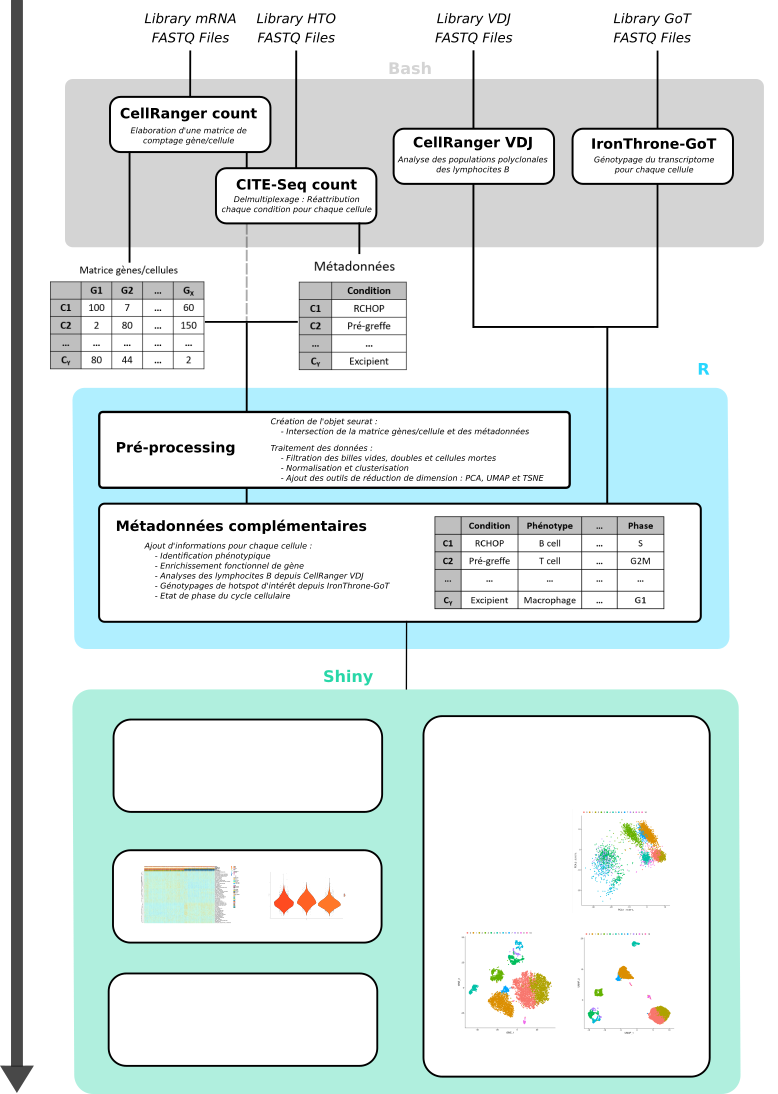
\includegraphics[scale=0.8]{figure/FL}
\caption{\small{Graphiques  \cite{1}.}}
\label{I1}
\end{figure}


%%%%%%%%%%%%%%%%%%%%%%%%%%%%%%%%%%%%%%%%%%%%%%%%%%%%%%%%%%%%%%%%%%%%%%%%%%%%%%%%%%%%%%%%%%%%%%%%%%%%%%%%%%%%%%%%%%%%%%%%%%%%%%%%%%%%%%%%%%%%%%%%%%%%%%%%%%%%%%%%%%%%%%%%%%%%%%%%%%%%%%%%%%%%%%%%%%%%%%%%%%%%%%%%%%%%%%%%%%%%%%%%%%%%%%%%%%%%%%%%%%%%%%%%%%%%%%%%%%%%%%%%%%%%%%%%%%%%%%%%%%%%%%%%%%%%%%%%%%%%%%%%%%%%%%%%%%%%%%%%%%%%%%%%%%%%%%%%%%%%%%%%%
\subsection{Résultats}
Une section présentant les résultats obtenus ;

\subsubsection*{1.}


\subsubsection*{2.}
%\begin{figure}[h!]
%   \begin{minipage}[c]{.46\linewidth}
%     \centering 
%     \includegraphics[scale=0.4]{figure/GSEA_tot1}
%     \caption{\small{Heatmap de corrélation des scores entre chacune des 19 activités en utilisant la méthode GSEA.}}
%     \label{I1}
%   \end{minipage} \hfill
%   \begin{minipage}[c]{.46\linewidth}
%     \centering 
%     \includegraphics[scale=0.4]{figure/AUC_tot1}
%     \caption{\small{Heatmap de corrélation des scores entre chacune des 19 activités en utilisant la méthode AUCell.}}
%     \label{I1}
%   \end{minipage}
%\end{figure}

%\begin{itemize}
%\item Groupe 1A : \textit{Blablabla}
%\end{itemize}

%\paragraph*{Relation entre activités et phase du cycle cellulaire.}


%%%%%%%%%%%%%%%%%%%%%%%%%%%%%%%%%%%%%%%%%%%%%%%%%%%%%%%%%%%%%%%%%%%%%%%%%%%%%%%%%%%%%%%%%%%%%%%%%%%%%%%%%%%%%%%%%%%%%%%%%%%%%%%%%%%%%%%%%%%%%%%%%%%%%%%%%%%%%%%%%%%%%%%%%%%%%%%%%%%%%%%%%%%%%%%%%%%%%%%%%%%%%%%%%%%%%%%%%%%%%%%%%%%%%%%%%%%%%%%%%%%%%%%%%%%%%%%%%%%%%%%%%%%%%%%%%%%%%%%%%%%%%%%%%%%%%%%%%%%%%%%%%%%%%%%%%%%%%%%%%%%%%%%%%%%%%%%%%%%%%%%%%
\subsection{Discussion}
Une section discussion qui contextualise les résultats par rapport à la problématique et au contexte général dans lequel s'inscrit le stage ;


%%%%%%%%%%%%%%%%%%%%%%%%%%%%%%%%%%%%%%%%%%%%%%%%%%%%%%%%%%%%%%%%%%%%%%%%%%%%%%%%%%%%%%%%%%%%%%%%%%%%%%%%%%%%%%%%%%%%%%%%%%%%%%%%%%%%%%%%%%%%%%%%%%%%%%%%%%%%%%%%%%%%%%%%%%%%%%%%%%%%%%%%%%%%%%%%%%%%%%%%%%%%%%%%%%%%%%%%%%%%%%%%%%%%%%%%%%%%%%%%%%%%%%%%%%%%%%%%%%%%%%%%%%%%%%%%%%%%%%%%%%%%%%%%%%%%%%%%%%%%%%%%%%%%%%%%%%%%%%%%%%%%%%%%%%%%%%%%%%%%%%%%%
\subsection{Conclusion}
Une conclusion qui présente également les perspectives ouvertes par le travail réalisé. 


%%%%%%%%%%%%%%%%%%%%%%%%%%%%%%%%%%%%%%%%%%%%%%%%%%%%%%%%%%%%%%%%%%%%%%%%%%%%%%%%%%%%%%%%%%%%%%%%%%%%%%%%%%%%%%%%%%%%%%%%%%%%%%%%%%%%%%%%%%%%%%%%%%%%%%%%%%%%%%%%%%%%%%%%%%%%%%%%%%%%%%%%%%%%%%%%%%%%%%%%%%%%%%%%%%%%%%%%%%%%%%%%%%%%%%%%%%%%%%%%%%%%%%%%%%%%%%%%%%%%%%%%%%%%%%%%%%%%%%%%%%%%%%%%%%%%%%%%%%%%%%%%%%%%%%%%%%%%%%%%%%%%%%%%%%%%%%%%%%%%%%%%%
%%% Votre page de biblio%%%%%
\addcontentsline{toc}{section}{4.Bibliographie}
\bibliographystyle{unsrt}
\renewcommand{\bibname}{\LARGE{\normalfont 4.~~\,\,\, B\textsc{ibliographie}}}
\vspace{-3cm}
\bibliography{mabiblio}
\end{document}